\documentclass{article}
\usepackage[left=1in, right=1in, top=1.3in, bottom=.8in]{geometry}
\usepackage{fancyhdr, amsfonts, amssymb, amsthm, MnSymbol, bbm, mathrsfs, graphicx, listings, parskip, hhline}
\pagestyle{fancy}
\def\Z{\mathbb{Z}}
\def\R{\mathbb{R}}
\def\Q{\mathbb{Q}}
\def\N{\mathbb{N}}
\def\C{\mathbb{C}}
\def\P{\mathbb{P}}
\def\E{\mathbb{E}}
\def\SF{\mathscr{F}}
\def\ind{\mathbbm{1}}
\def\giv{{\,|\,}}
\def\lf{\left\lfloor}
\def\rf{\right\rfloor}
\def\lc{\left\lceil}
\def\rc{\right\rceil}
\def\eqd{ \stackrel{d}{=} }
\def\p{ \stackrel{\P}{\rightarrow} }
\def\as{ \stackrel{as}{\rightarrow} }
\def\d{ \stackrel{d}{\rightarrow} }
\def\w{ \stackrel{w}{\rightarrow} }
\def\v{ \stackrel{v}{\rightarrow} }

% 3x3 matrix code
% $$ \left( \begin{array}{ccc}
% a & b & c \\
% d & e & f \\
% g & h & i \end{array} \right)$$

% formula in array
% $$ |x| = \left\{ \begin{array}{ll}
%        x & \mbox{if $x \geq 0$};\\
%        -x & \mbox{if $x < 0$}. \end{array} \right. $$

\title{Twitter Sentiment Analysis}
\author{Eric Kim, Jonathan Wang}
\date{}

\begin{document}
\maketitle

\section{Exploratory Data Analysis}

\subsection{Introduction}
Predicting tweet sentiment is an area with many applications beyond just Twitter. Of course, it helps Twitter to improve its services in many ways. For instance, if Twitter determines that most of a user's tweets are of positive sentiment, it is not unreasonable to believe that a particular user may not benefit or seek to benefit from negative sentiment tweets and can filter up positive sentiment tweets for such a user. Another example is that we can further analyze positive and negative tweets. That is, once we have a good method of finding negative sentiment tweets, we might start rank the tweets on now negative these are. If we can identify a negative tweet to be threatening, for instance, Twitter might be able to contact relevant authorities to prevent an incident.

However, tweet sentiment analysis is useful for work outside of Twitter. Looking at work of Bollen, Mao [1], we see that tweet sentiment has been used for predicting stocks, which is not at all obviously related to tweet sentiment. This highlights some of the importance of tweet sentiment because of its connections beyond Twitter.

Our data of interest that we examine consists of 50000 tweets with 1000 predictors of the most commonly seen words on twitter. The response is binary and tells us the sentiment of the tweet - either good or bad. We use this dataset to make predictions and submit to Kaggle. %An expanded dataset with 1.4 million tweets includes the actual tweets, and this dataset will used for feature engineering. When model fitting, we will fit and predict both with and without these features.

\subsection{Data Cleaning}
One thing to be particularly wary about is white noise in the data. In particular, these are tweets whose predictors add no value for the purposes of predictions. One example of these type of white noise tweets are those with $0$'s in each of the 1000 predictors since predicting the sentiment of the tweet with no predictors is tantamount to flipping a coin. In the smaller dataset with 50000 tweets, we find 288 of these and proceed to remove them.

Referencing the work of Pang et. al [2], we have that feature presence is more useful than feature frequency so we create a binary matrix of the initial features and compare all of the following methods with both the original data and the binary data.

Furthermore, this dataset is filled with a lot of stop word predictors. These are words that add no particular value to the predictors, that is, they amount to not much more than white noise. To reduce this white noise and speed up computation time, we use the \texttt{tm} package to remove these stop words. We further clean out the singular alphabetical letters (e.g. ``a'', ``b'', ``c'', ...). 

We also clean out the punctuation. While there are merits to including some in sentiment analysis (e.g. multiple !!!! in a row), since we binarize the data, this information is lost. However, since exclamation marks can be used in both positive and negative ways, we leave these cleaned out to avoid ambiguity. %However in the feature engineering section, we will reincorporate these features back.

Finally, we also remove any unicode characters since they too amount to white noise in the predictor set. For example, a > does not differentiate much from ? aside from the fact that in Spanish, starting a sentence with > indicates that ? will conclude the sentence. 

Since we have cleaned up a lot of predictors, we are bound to have newly introduced some white noise tweets. We clean these out as well so that we end up with a compact dataset which features the most important words driving tweet sentiment and ignores as much white noise as possible.

Finally, for the sake of comparison, we will fit models on three different datasets. The full dataset with minimal cleaning of the rows with no entries in any of the predictors, the cleaned dataset as described above, and then a binarized dataset after the cleaning. These three datasets should allows us to get a good grasp on how the cleaning affected our results.

\subsection{Data Exploration}
First, we take a look at which words are most connected with positive sentiment tweets and negative sentiment tweets. To see further why we would need to clean out some of the stop words, we look at the whole data first. 

Of the top 50 words that showed up in the positive tweets for the whole data, we see \texttt{love} 1340 times, \texttt{thanks} 1116 times, and \texttt{lol} 1058 times. Of the top 50 words after cleaning, we see \texttt{good} 1388 times, \texttt{love} 935 times, \texttt{lol} 873 times, \texttt{thanks} 649 times, \texttt{hope} 510 times, \texttt{great} 495 times, \texttt{haha} 471 times, \texttt{wish} 437 times, and \texttt{fun} 422 times. So just from a little bit of cleaning, we have retrieved more information from the data. However, one thing to note is that of the top 50, \texttt{bad} showed up 451 times and \texttt{sad} showed up 448 times. So although the words we would guess are associated with positive sentiment showed up a lot, we also find words associated with negative sentiment show up quite a bit as well.

Doing a similar analysis for the negative sentiments, we find \texttt{oh} 629 times, \texttt{miss} 534 times, \texttt{sorry} 451 times, and \texttt{sad} 429 times. However, this portion of the data is less informative since \texttt{good}, \texttt{love}, \texttt{lol}, \texttt{thanks}, \texttt{great}, \texttt{hope}, \texttt{haha}, \texttt{wish}, and \texttt{fun} all show up in the top 50. This is indicative of the fact that some words we think of as positive can also be used in a negative manner. For instance, words like \texttt{love}, \texttt{lol}, and \texttt{haha} can be used in a sarcastic tone, which often is associated with a negative context.

%\section{Feature Engineering}

\section{Hyperparameter Tuning}
For each of these methods, we use one model (typically the binarized one) to manually tune the hyperparameters. After finding a hyperparameter that approximately maximizes our CV Accuracy, we use this hyperparameter for all three datasets.

\subsection{$L^1$ Penalized Logistic Regression}
We used \texttt{cv.glmnet} to get \texttt{lambda.min}, which is the $\lambda$, which we report in the next section. The following are plots of the mean cross validated error against the varying $\lambda$ values that \texttt{cv.glmnet} tried. \\

\centerline{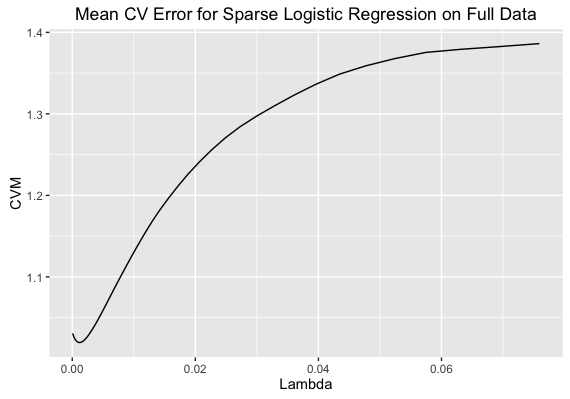
\includegraphics[scale=.25]{diagrams/1logreg.png} ~~~ 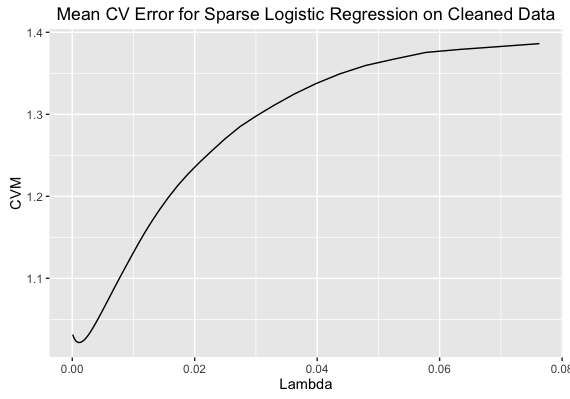
\includegraphics[scale=.25]{diagrams/2logreg.png} ~~~ 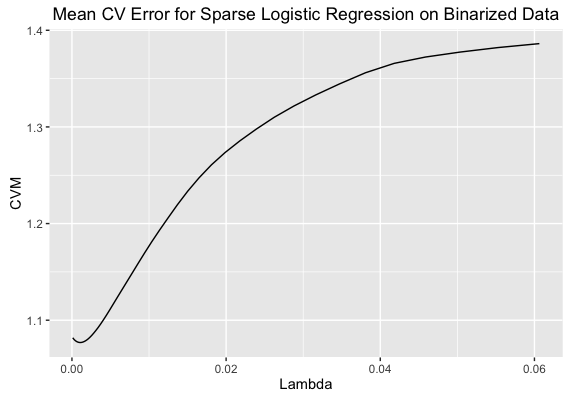
\includegraphics[scale=.25]{diagrams/3logreg.png}}

\subsection{Random Forest}
For random forests, we fit a model with 100, 500, 1000, and 1500 trees. Interestingly enough, the fits with 500 and 1000 trees performed worse than the model with 100 trees. The following are plots of the misclassification error and the F1 Score. When fitting our model in the next section, we fit with 100 trees instead of 1500 trees in order to prioritize runtime efficiency and because their CV accuracy and  F1 scores were similar. \\

\centerline{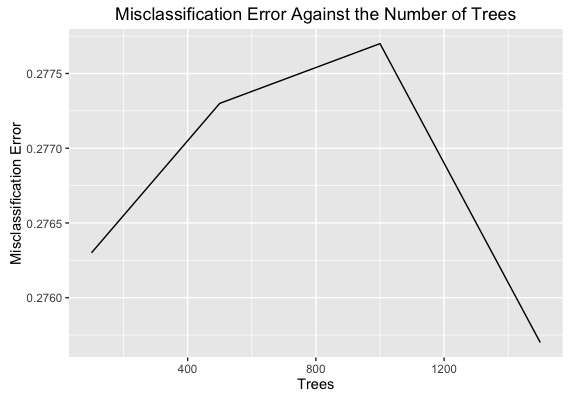
\includegraphics[scale=.29]{diagrams/6rf.png} ~~~~~~~~~~~~~~~ 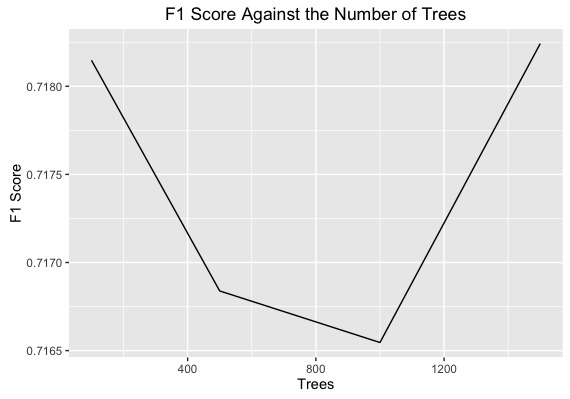
\includegraphics[scale=.29]{diagrams/7rf.png}}

\subsection{Generalized Boosting Models}
For the GBM models, we used Adaboost with the following fixed hyperparameters \texttt{interaction.depth=5} and \texttt{shrinkage=.01}. We tried \texttt{n.trees=500,1000,1500,2000} on the binarized data. Toward the larger tree sizes, \texttt{gbm} runs slower, but not as slow as Random Forests so we fit the other models with 2000 trees even though it performed similarly to 1500 trees. \\

\centerline{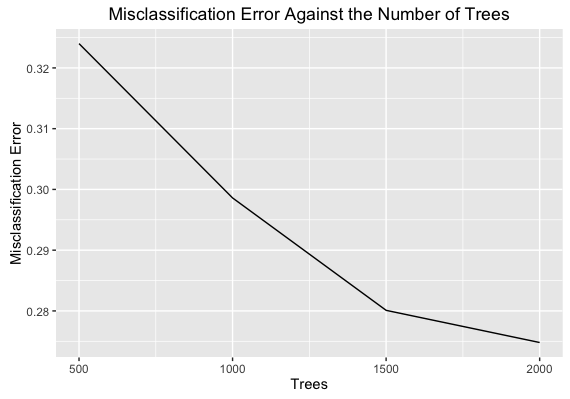
\includegraphics[scale=.29]{diagrams/4gbm.png} ~~~~~~~~~~~~~~~ 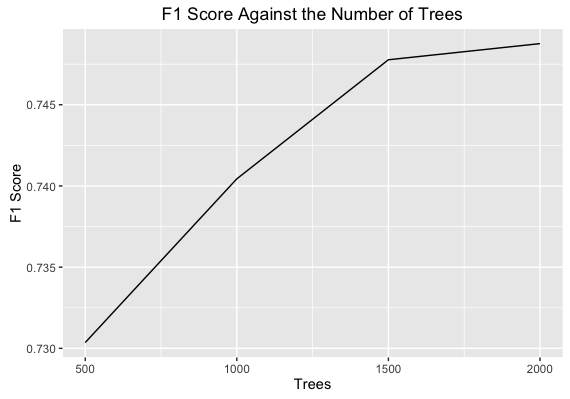
\includegraphics[scale=.29]{diagrams/5gbm.png}}

\subsection{Neural Networks}
Due to the sheer computational cost of running neural nets, we only fit models with 200 neurons and 500 neurons, and only on the cleaned, binarized dataset. As we see, they performed very similarly. Also due to the submission limitations of Kaggle, we were unable to submit neural net results to Kaggle. \\

\centerline{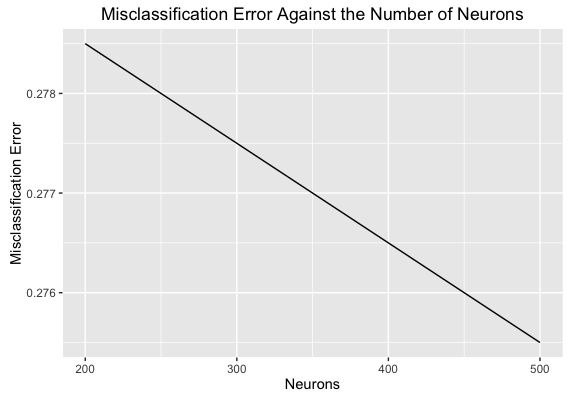
\includegraphics[scale=.29]{diagrams/8nn.png} ~~~~~~~~~~~~~~~ 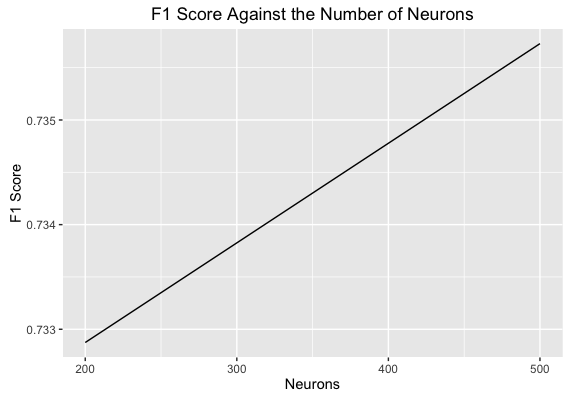
\includegraphics[scale=.29]{diagrams/9nn.png}}

\section{Model Fitting}
For our models, we focus on four methods: logistic regression, random forest, gradient boosting, and neural networks. These models were chosen because of their capabilities for classification. We present the results in the tables below. To cross validate, we trained our model to all but 10000 data points in their respective models and looked at the CV Accuracy as well as the CV F1 Score and report those below as well. Also due to limitations in Kaggle submissions, we take the dataset with the best CV Accuracy and submit that to Kaggle.

\subsection{$L^1$ Penalized Logistic Regression}
$$\begin{array}{|c|c|c|c|c|}
\hline
\text{Model} & \text{CV Acc} & \text{Kaggle Acc} & \text{CV F1 Score} & \text{Hyper-Parameters} \\
\hhline{|=|=|=|=|=|}
\text{Logistic Regression} & 0.7576 & 0.75844 & 0.7640936 & \lambda = 0.001153669\\
\hline
\text{Cleaned LR} & 0.7324 & - & 0.7458752 & \lambda = 0.001159524 \\
\hline
\text{Binarized LR} & 0.7314 & - & 0.7445311 & \lambda = 0.001110128 \\
\hline
\end{array}$$

\subsection{Random Forest}
$$\begin{array}{|c|c|c|c|c|}
\hline
\text{Model} & \text{CV Acc} & \text{Kaggle Acc} & \text{CV F1 Score} & \text{Hyper-Parameters}   \\
\hhline{|=|=|=|=|=|}
\text{Random Forest} & 0.7455 & 0.70640 & 0.7393782 & \text{n.trees} = 100 \\
\hline
\text{Cleaned RF} & .7241 & - & 0.7177337 & \text{n.trees} = 100 \\
\hline
\text{Binarized RF} & 0.7237 & - & 0.7181475 & \text{n.trees} = 100 \\
\hline
\end{array}$$

\subsection{Generalized Boosting Models}
$$\begin{array}{|c|c|c|c|c|}
\hline
\text{Model} & \text{CV Acc} & \text{Kaggle Acc} & \text{CV F1 Score} & \text{Hyper-Parameters} \\
\hhline{|=|=|=|=|=|}
\text{Gradient Boosting} &0.73429  & - & 0.7453392 & \text{n.trees} = 2000 \\
\hline
\text{Cleaned GB} & 0.73858 & 0.70700 & 0.7466003 & \text{n.trees} = 2000 \\
\hline
\text{Binarized GB} & 0.7252 & - & 0.7487658 & \text{n.trees} = 2000 \\
\hline
\end{array}$$

\subsection{Neural Networks}
$$\begin{array}{|c|c|c|c|c|}
\hline
\text{Model} & \text{CV Acc} & \text{Kaggle Acc} & \text{CV F1 Score} & \text{Hyper-Parameters} \\
\hhline{|=|=|=|=|=|}
\text{Binarized Neural Network } & 0.7245 & - & 0.7357298 & \text{neurons} = 200 \\
\hline
\end{array}$$

\subsection{Comparison}
It seems that the $L^1$ Penalized Logistic Regression performed the best, much to our surprise. It had the fastest runtime (at most a few minutes on a 6 year old computer) and with no adjustments, performed better than the other methods as well as with all the cleaned adjustments. The remaining three performed approximately similarly at around $72\%$ for the CV Accuracy and $70\%$ for the Kaggle Accuracy. This suggests that perhaps we should have cleaned less and added more meaningful predictors. Due to time restrictions and inexperience in Python, we have elected to skip feature engineering, however, should we come back to this dataset, feature engineering definitely seems necessary to push beyond $76\%$. To conclude, we perform some ensembles, which we will see will perform quite well.

\section{Ensemble}
To conclude, we will perform some ensembles. First, since the $L^1$ Penalized Logistic Regression performed so well, we so an ensemble of five of them with the full robust dataset using five different seeds for the models. Then, since these were the first three models that finished running, we ensembled the $L^1$ Penalized Logistic Regression with the full dataset, Random Forest with the binarized dataset, and the Generalized Boosting Models with the binarized dataset. For our final ensemble, we ensembled two $L^1$ Penalized Logistic Regression on the full dataset and one of each of the rest on the binarized dataset. The reason for using two of the Logistic Regression is because they peformed better so we wanted to add more weight to their decisions. The method of prediction was majority vote. That is, each model would predict on their own then would vote on the response. The results are reported below.

$$\begin{array}{|c|c|c|c|}
\hline
\text{Model} & \text{CV Acc} & \text{Kaggle Acc} & \text{F1 Score} \\
\hhline{|=|=|=|=|}
\text{5$\times$ LR} & 0.7722 & 0.75388 & 0.7644621 \\
\hline
\text{LR + RF + GBM} & 0.7809 & 0.73420 & 0.7557563 \\
\hline
\text{$2\times$ LR + RF + GBM + NN} & 0.8026 & 0.73548 & 0.823 \\
\hline
\end{array}$$


\section{Conclusion}
In conclusion, we were unable to do better than just running a $L^1$ Penalized L
ogistic Regression on a minorly cleaned dataset. It seemed like we might have cl
eaned too many predictors and certainly feature engineering would have helped in
 our predictions. Some of our methods took many hours to run and that did not he
lp when trying to cross validate. At the end, we found that our ensembling perfo
rmed particularly well when cross validating, getting up to 80\% at one point. A
nd even though our ensembled models were for the most part higher than our other
 models when submitting on Kaggle, it did not perform as we hoped. Perhaps in th
e ensembling, there was overfitting and hence we saw much better results in our
data than on Kaggle. All in all, if we were to return to this dataset or work wi
th similar datasets, it seems feature engineering would play a rather large role
 in improving accuracy.

\section{References}
[1] J. Bollen and H. Mao. Twitter mood as a stock market predictor. IEEE Computer, 44(10):91–94, (2010)

[2] Pang, B., Lee, L., Vaithyanathan, S.: Thumbs up?: sentiment classification using machine
learning techniques, pp. 79–86 (2002)

[GITHUB] https://github.com/ericaaronkim/tweetpredictors
\end{document}
